\begin{titlepage}
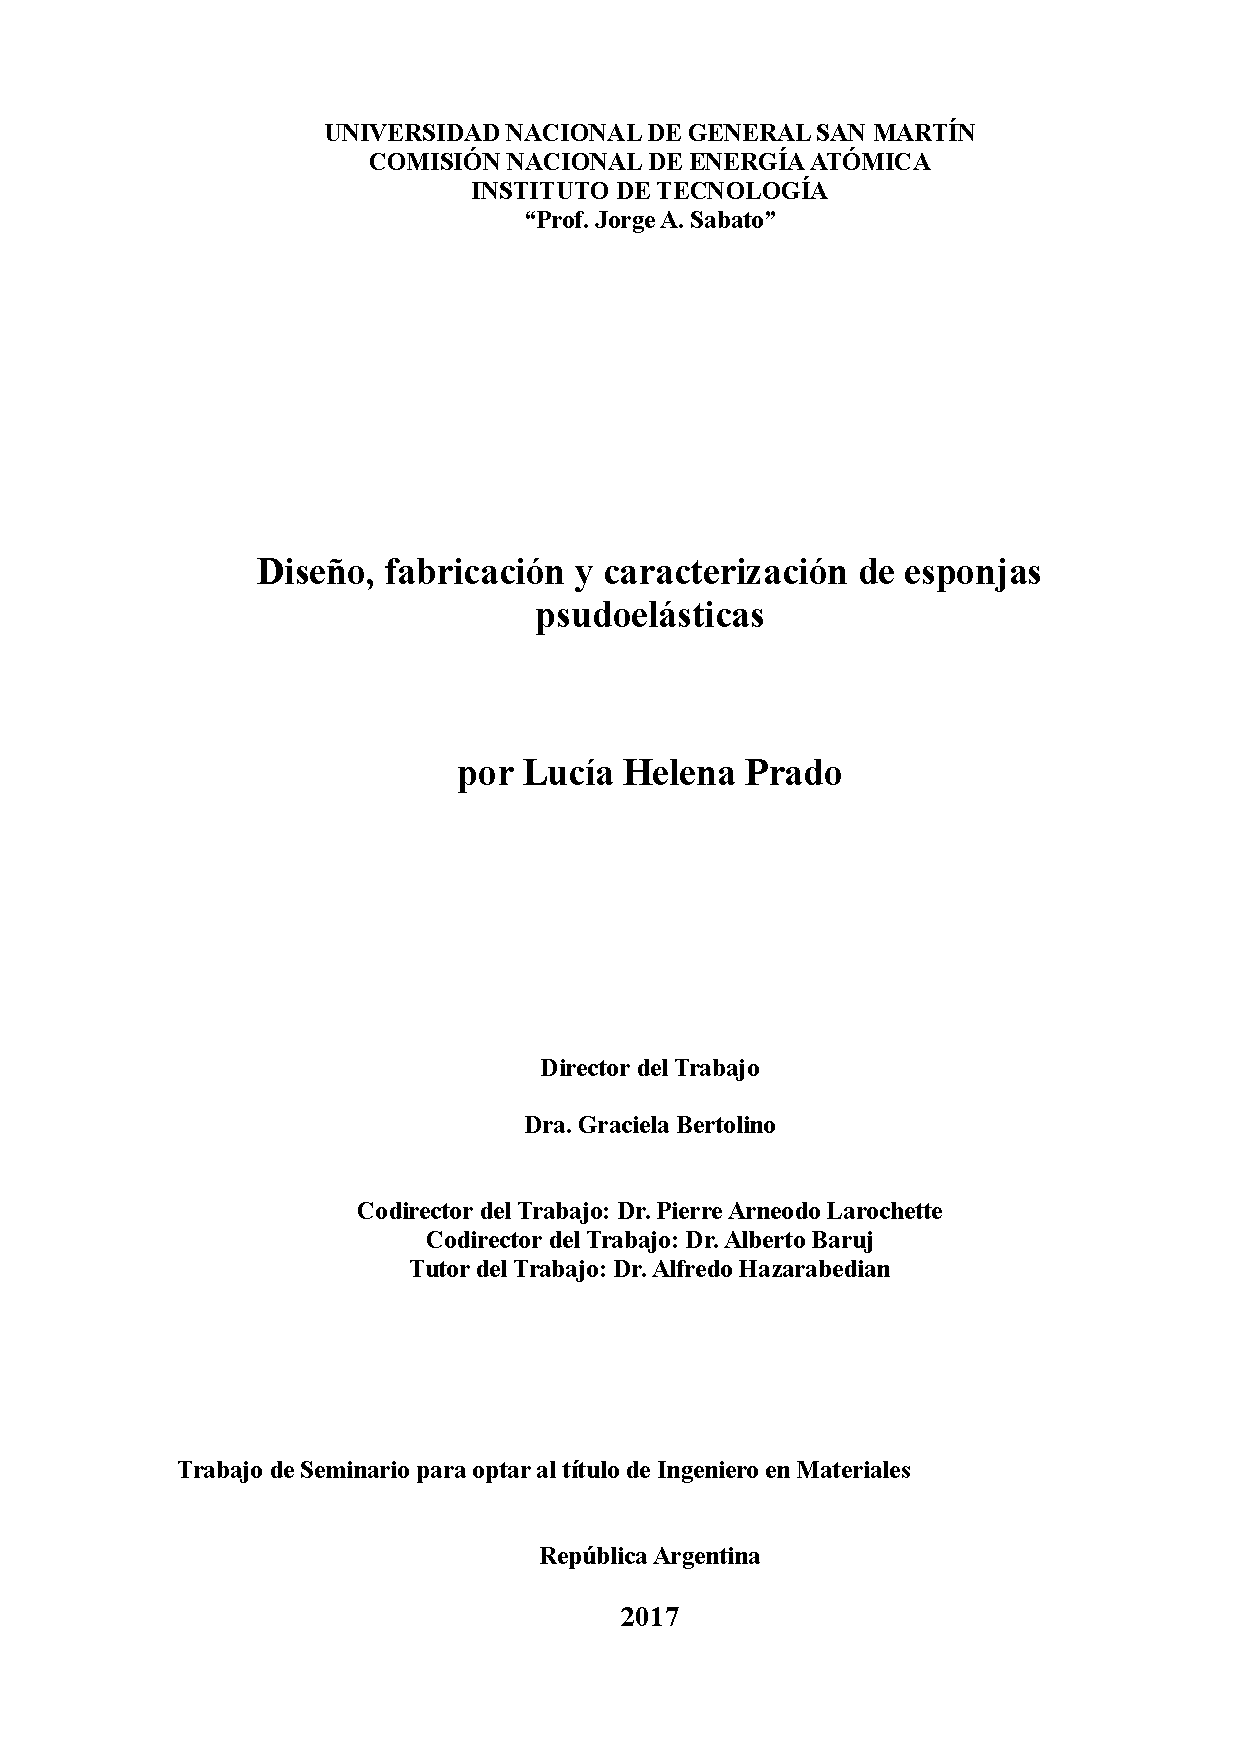
\includepdf[page={-},offset=0mm 0mm]{Img/caratula_is.pdf}
\end{titlepage}

\thispagestyle{empty}
\cleardoublepage

\begin{titlepage}
\begin{flushright}
\large \sffamily

\vspace*{-1.7cm}
% Logo mini de la facultad arriba a la derecha

\includegraphics[width=.2\textwidth]{Img/logo_is.jpg}\\[2cm]
% Logo de la facultad arriba a la izquierda
% \begin{flushleft}
% \includegraphics[width=.6\textwidth]{fiuba.pdf}\\[2cm]
% \end{flushleft}

% Título
\begin{huge}
\bfseries
\textbf{Diseño, fabricación y caracterización de esponjas psudoelásticas}\par
\end{huge}
% {\Large \bfseries
% Técnicas de cooperación en redes de sensores: Transmisión cooperativa mediante
% OSTBC}\\
\rule{\linewidth}{1.5mm}\\[0.1cm]
\textsc{Seminario de Ingeniería en Materiales}\\[2.5cm]

% Autor y director
{\small autor:}
Lucía Helena \textsc{Prado}\\

\vspace{10mm}
{\small directora:}
Dra. Graciela \textsc{Bertolino} \\
{\small codirectores:}
Dr. Pierre \textsc{Arneodo Larochette} \\
Dr. Alberto \textsc{Baruj} \\
{\small tutor:}
Dr. Alfredo \textsc{Hazarabedian} \\


% Lugar y fecha al final
\begin{table*}[b]
\flushbottom
\centering \sffamily %\scshape \large
\textsc{República Argentina}\\[1mm]
\today
\end{table*}

\end{flushright}
\end{titlepage}

\thispagestyle{empty}
\cleardoublepage